\documentclass[xcolor=dvipsnames, 14pt]{beamer}
\usetheme{Darmstadt}
\usecolortheme[named=LimeGreen]{structure}

% balíčky

\usepackage[utf8]{inputenc}
\usepackage[czech]{babel}
\usepackage{graphicx}

% informace o dokumentu

\title[Synchronization and replication of geodata]{Synchronization and replication \\ of geodata in the Esri platform}
\author[M. Solanská]{Markéta Solanská}
\date[6.11.2013]{6.11.2013}


% text dokumentu

\begin{document}

% titulní stránka
% (název prezentace, autor, datum...)

\begin{frame}
  \titlepage
\end{frame}

% osnova prezentace
% (většinou se pro délku vypouští)

% obsah prezentace
% (používají se klasické sekce)

\section{Synchronization and replication of geodata in the Esri platform}

  \begin{frame}
    \frametitle{Main goals}
    \framesubtitle{Theoretical part}
    \begin{itemize}
      \item definition of the synchonization and replication processes
      \item description of replication possibilities, types and properties
      \item description of solutions for different types of tasks
    \end{itemize}
  \end{frame}

  \begin{frame}
    \frametitle{Main goals}
    \framesubtitle{Practical part}
    \begin{itemize}
      \item practical test of replication for different data types and different types of tasks
      \item test: speed, completeness, accuracy, quality of transferred data, formats
      \item databases: PostgreSQL 9.x + PostGIS
      \item ERSI products: ArcSDE + ArcGIS for Desktop or ArcGIS for Server
    \end{itemize}
  \end{frame}

  \begin{frame}
    \frametitle{Replication}
    \begin{itemize}
      \item copying and distribution of data and database objects from server to another
      \item means full copy of data and then synchonizate of changes
      \item main reasons for replication:
        \begin{itemize}
        \begin{normalsize}
          \item high availability
          \item data movement
          \item sharing data across the users
        \end{normalsize}
        \end{itemize}
      \item synchronous x asynchronous replication
      \item one-way x two-way replication
    \end{itemize} 
  \end{frame}

  \begin{frame}
    \frametitle{Replication}
    \begin{itemize}
      \item master-slave replication
      \\  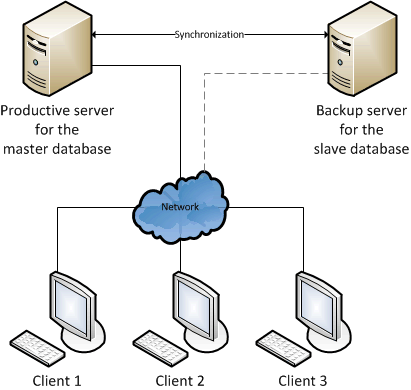
\includegraphics[scale=0.5]{obr/db_replikation.png} 
      \\  \begin{tiny}(zdroj:http://www.passwordsafe.de/uploads/pics/db\_replikation\_EN.gif)\end{tiny}
    \end{itemize} 
  \end{frame}

  \begin{frame}
    \frametitle{ArcSDE Technology}
    \framesubtitle{ESRI product}
    \begin{itemize}
        \item middle-ware for communitacion between user and SQL database (example. ArcGIS for Desktop and PostgreSQL)
        \item for managing spatial data in relational database system
        \item multi-user editing
        \item support for PostgreSQL
    \end{itemize} 
  \end{frame}

  \begin{frame}
    \frametitle{Results of the diploma thesis}
    \begin{itemize}
      \item description of the replication and synchronization processes and their requirements for Ersi products
      \item manual how to configure replication
      \item evaluation of replication process depend on speed, quiality, completness, ..
    \end{itemize}
  \end{frame}
  
  \begin{frame}
    \frametitle{What I've already did?}
    \begin{itemize}
      \item set up replication on two computers: \\ both WIN XP + pgAdmin3 + Slony-I
      \item Slony-I is plugin for master-slave replication
      \item visualization in the QGIS
      \item data set: simple vector data 
    \end{itemize}
  \end{frame}


\end{document}
